\begin{figure}[h]
    \centering
    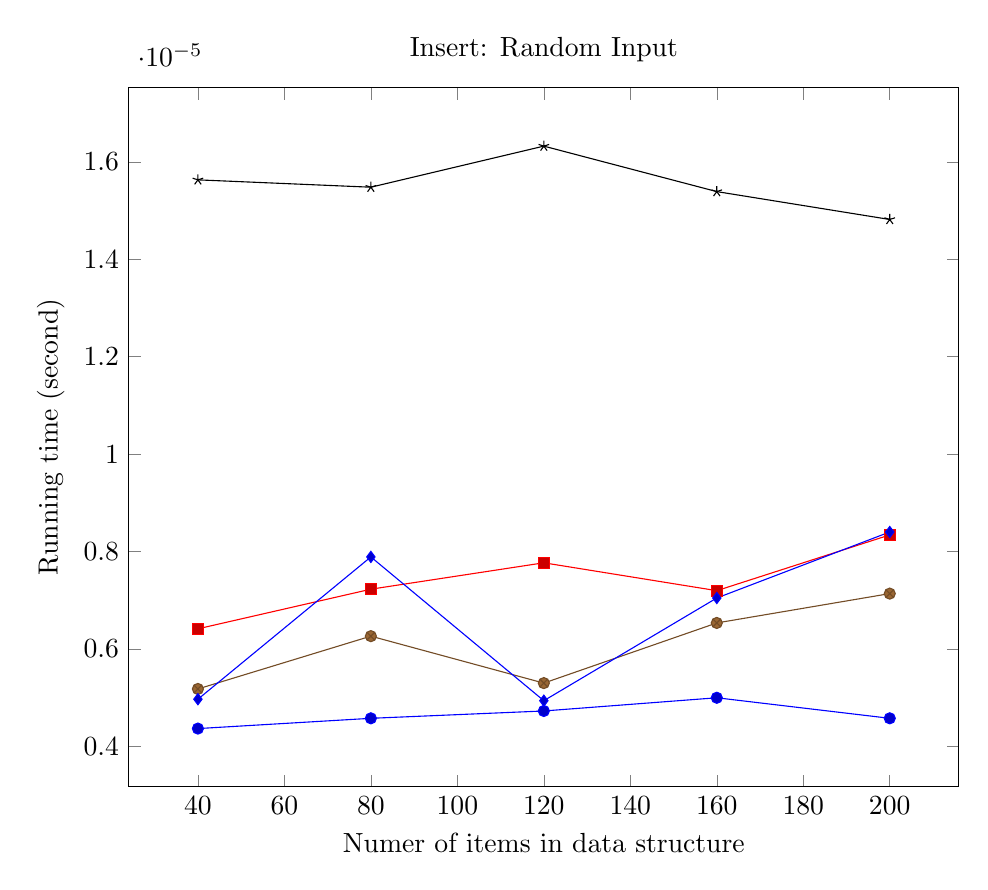
\begin{tikzpicture}
        \begin{axis}[
            xlabel={Numer of items in data structure},
            ylabel={Running time (second)},
            title={Insert: Random Input},
            width=\textwidth
        ]
		\addplot coordinates {
			(40, 4.367042383179864e-06)
			(80, 4.577865118804425e-06)
			(120, 4.728452787006176e-06)
			(160, 4.999510590053547e-06)
			(200, 4.577865118804425e-06)
		};
		\addplot coordinates {
			(40, 6.415034672713204e-06)
			(80, 7.228208081855314e-06)
			(120, 7.770323687950053e-06)
			(160, 7.198090548499181e-06)
			(200, 8.342556827756199e-06)
		};
		\addplot coordinates {
			(40, 5.180215791966703e-06)
			(80, 6.264447004511453e-06)
			(120, 5.300685926812321e-06)
			(160, 6.535504807558823e-06)
			(200, 7.1378554810763715e-06)
		};
		\addplot coordinates {
			(40, 1.5630999977389594e-05)
			(80, 1.548041230918784e-05)
			(120, 1.6323703251686085e-05)
			(160, 1.5390059708053626e-05)
			(200, 1.4817826568247482e-05)
		};
		\addplot coordinates {
			(40, 4.969393056342142e-06)
			(80, 7.890793822795672e-06)
			(120, 4.939275522630737e-06)
			(160, 7.047502879942158e-06)
			(200, 8.402791895534278e-06)
		};
        \legend{}
        \end{axis}
    \end{tikzpicture}
    \caption{Average of 0 operations, benchmarked every 0, starting at 0.}
\end{figure}